%%%%%%%%%%%%%%%%%%% vorlage.tex %%%%%%%%%%%%%%%%%%%%%%%%%%%%%
%
% Beispiel-Vorlage zur Erstellung von Projekt-Dokumentationen
%
% Benutzen Sie bitte diese Datei um Ihre Dokumente zu erstellen
%
%%%%%% erstellt anhand svmono-Springer-Verlag-Vorlage %%%%%%%%%


%%%%%%%%%%%%%%%%%%%%%%%%%%%%%%%%%%%%%%%%%%%%%%%%%%%
\documentclass[envcountsame,envcountchap,deutsch]{i-studis}
\usepackage{makeidx}   % Erlaubt die Erzeugung eines Index-Verzeichnisses
\usepackage{multicol}  % Zweispaltiger Index-Verzeichnis
%\usepackage[bottom]{footmisc} % Erzeugung von Fußnoten nur beim Bedarf einbinden

%%--------------------------------------------------------
\usepackage[pdftex]{graphicx}
\usepackage[pdftex,plainpages=false]{hyperref}
%%-----------------------------------------------------
\usepackage{color}	    % Farbverwaltung
% \usepackage{ngerman}     % Neue deutsche Rechtsschreibung
\usepackage[T1]{fontenc} % Silbentrennung 
\usepackage[english, ngerman]{babel}
% Alle eingebundenen Dateien sollten die passenden Encodings haben
% \usepackage[ansinew]{inputenc}  % Umlaute für Windows (öäüß)
% \usepackage[latin1]{inputenc}   % Umlaute für Linux
% \usepackage[applemac]{inputenc} % Umlaute für Mac
\usepackage[utf8]{inputenc}     % generelle Umlaute-Darstellung
%-----------------------------------------------------
\usepackage{listings} % Optionen für Code-Darstellung
\lstset
{% general command to set parameter(s)
	basicstyle=\scriptsize, % print whole listing small
	keywordstyle=\color{blue}\bfseries,
	% underlined bold black keywords
	identifierstyle=, % nothing happens
	commentstyle=\color{white}, % white comments
	stringstyle=\ttfamily, % typewriter type for strings
	showstringspaces=false, % no special string spaces
	framexleftmargin=7mm, 
	tabsize=3,
	showtabs=false,
	frame=single, 
	rulesepcolor=\color{blue},
	numbers=left,
	linewidth=146mm,
	xleftmargin=8mm
}
\usepackage{textcomp} % celsius - Darstellung
\usepackage{
	amssymb,
	amsfonts,
	amstext,
	amsmath
} % Mathematische Symbole
\usepackage[german, ruled, vlined]{algorithm2e}
\usepackage[a4paper]{geometry} %Andere Formatierung
\usepackage{bibgerm}
\usepackage{array}
\hyphenation{Test-ein-gabe} %Silbentrennung bei falschen Trennung anfügen
\setlength{\textheight}{1.1\textheight}
\pagestyle{myheadings} % Erzeugt selbstdefinierte Kopfzeile
\makeindex % Index-Erstellung

% Ab hier beginnt das eigentliche Dokument.
%--------------------------------------------------------------------------
\begin{document}

%------------------------- Titelblatt -------------------------------------
\title{Titel der Projekt- Abschlussarbeit auf Deutsch}
\subtitle{English Title of Project Work}
%---- Die Art der Dokumentation kann hier ausgewählt werden---------------
%\project{Master Abschlussarbeit}
%\project{Master Projektstudium}
%\project{Bachelor Abschlussarbeit}
\project{Projektarbeit}
%\project{Seminar zur Vorlesung ...}
% \project{Hausarbeit zur Vorlesung ...}
%--------------------------------------------------------------------------
\supervisor{Titel Vorname Name} % Betreuer der Arbeit
\author{Autor}                  % Autor der Arbeit
\address{Ort, den}              % hier wird der Ort eingetragen
\submitdate{Abgabedatum}        % Abgabedatum \today :)

\begingroup
  \renewcommand{\thepage}{Titel}
  \mytitlepage
  \newpage
\endgroup
%--------------------------------------------------------------------------
\frontmatter 
%--------------------------------------------------------------------------
\danksagung

Dank an ... %Danksagungen
\preface

Ein Vorwort ist nicht unbedingt nötig. Falls Sie ein Vorwort schreiben, so ist dies der Platz, um z.B. die Firma vorzustellen, in der diese Arbeit entstanden ist, oder einigen Leuten zu danken, die in irgendeiner Form positiv zur Entstehung dieser Arbeit beigetragen haben. Auf keinen Fall sollten Sie im Vorwort die Aufgabenstellung näher erläutern oder vertieft auf technische Sachverhalte eingehen.

\kurzfassung
Hier soll eine Kurzfassung der Arbeit stehen. Eine halbe Seite sollte genügen. Die Kurzfassung gibt in einer verständlichen Form den Gegenstand und das Ergebnis der Arbeit an. Sie soll dem Leser vermitteln, um was es geht und was die Leistung der Arbeit ist. Damit kann der Leser entscheiden, ob Thema, Inhalt und Ergebnis der Arbeit für ihn so interessant sind, dass er sie liest.
\\[3ex]
\noindent
The same in english (optional).

 % Kurzfassung Deutsch/English
\tableofcontents %Inhaltsverzeichnis - notwendig
% \listoffigures % Abbildungsverzeichnis - optional
% \listoftables % Tabellenverzeichnis- optional
%--------------------------------------------------------------------------
\mainmatter                     %Hauptteil (ab hier in arab. Seitenzahlen)
%--------------------------------------------------------------------------
% Kapitell werden einzeln abgespeichert und hier eingefügt
\chapter{Einleitung}

Begonnen werden soll mit einer Einleitung zum Thema: z.B. Hintergrund und Ziel (was, warum).

\chapter{Problemstellung}

Hier wird i.d.R. zunächst das generell vorliegende Problem diskutiert: Was ist zu lösen - was gibt es bisher an Lösungsansätzen (prinzipiell) und warum ist es wichtig, dass man dieses Problem löst. Letzteres ergibt sich oftmals aus der vorliegenden Anwendungssituation: Man braucht die Lösung, um eine bestimmte Aufgabe zu erledigen, ein System aufzubauen etc. Der Bezug auf vorhandene oder auch bisher fehlende Lösungen begründet auch die Intension und Bedeutung dieser Arbeit. Dies können allgemeine Gesichtspunkte sein - man liefert einen Beitrag für ein generell erkanntes oder zu erkennendes Problem - oder man hat eben eine spezielle Systemumgebung oder Produkt (z.B. in einer Firma u.s.w.), woraus sich dieses noch zu lösende Problem ergibt.

Die genaue Problematik und Randbedingungen werden dann in Kapitel \hyperref[Aufgabenstellung]{Kapitel~\ref{Aufgabenstellung}}
dargestellt.

\chapter{Aufgabenstellung und Zielsetzung}\label{Aufgabenstellung}

Hier wird nun die Aufgabenstellung konkret dargestellt: Was ist spezifisch zu lösen? Welche Randbedingungen sind prinzipiell gegeben und was ist die Zielsetzung? Letztere soll das beschreiben, was man mit dieser Arbeit (mindestens) erreichen möchte.
\chapter{Übrige Abschnitte (Kapitel und Absätze)}
Die Gliederung hängt natürlich vom Thema und von der Lösungsstrategie ab. Als nützliche Anhaltspunkte können die Entwicklungsstufen oder - schritte z.B. der Softwareentwicklung betrachtet werden. Nützliche Gesichtspunkte erhält und erkennt man, wenn man sich
\begin{itemize}
  \item in die Rolle des Lesers oder
  \item in die Rolle des Entwicklers, der die Arbeit z.B. fortsetzen, ergänzen oder pflegen soll,
\end{itemize}
versetzt. In der Regel wird vorausgesetzt, dass die Leser einen fachlichen Hintergrund haben - z.B. Informatik studiert haben. D.h. nur in besonderen, abgesprochenen Fällen schreibt man in populärer Sprache, so dass auch Nicht-Fachleute die Ausarbeitung prinzipiell lesen und verstehen können.

Die äußere Gestaltung der Ausarbeitung hinsichtlich Abschnittformate, Abbildungen, mathematische Formeln usw. wird in \hyperref[Stile]{Kapitel~\ref*{Stile}} kurz dargestellt.
\chapter{Latex-Bausteine}\label{Stile}

Der Text wird in bis zu drei Ebenen gegliedert:

\begin{enumerate}
  \item Kapitel ( \verb \chapter{Kapitel} ), \index{Kapitel}
  \item Unterkapitel  (  \\section{Abschnitt} ) und
  \item Unterunterkapitel  ( \\subsection{Unterabschnitte} ).
\end{enumerate}

\section{Abschnitt}\index{Abschnitt}
Text der Gliederungsebene 2.


\subsection{Unterabschnitt} \index{Unterabschnitt}
Text der Gliederungsebene 3. Text Text Text Text Text Text Text Text Text Text Text Text Text Text Text. Beispiel für Quelltext\index{Quelltext} \\[2 ex]
\noindent
\begin{minipage}{1.0\textwidth} \small
	\begin{lstlisting}
		Prozess 1:
	
		Acquire();
			a := 1;
		Release();
		...
		Acquire();
		if(b == 0)
		{					
			c := 3;
			d := a;
		}				
		Release();
	\end{lstlisting}
\end{minipage}

\vspace{2cm}
\noindent
\begin{minipage}{1.0\textwidth} \small
	\begin{lstlisting}
		Prozess 2:
	
		Acquire();
			b := 1;
		Release();
		...
		Acquire();
		if(a == 0)
		{					
			c := 5;
			d := b;
		}				
		Release();
	\end{lstlisting}
\end{minipage}
\vskip 1em

Größere Code-Fragmente sollten im Anhang eingefügt werden.

\section{Abbildungen und Tabellen}

Abbildungen\index{Abbildung} und Tabellen\index{Tabelle} werden zentriert eingefügt. Grundsätzlich sollen sie erst dann erscheinen, nach dem sie im Text angesprochen wurden (siehe Abb. \ref{a1}). Abbildungen und Tabellen (siehe Tabelle \ref{t1}) können im (fließenden) Text ( here ), am Seitenanfang (\verb top ), am Seitenende (\verb bottom ) oder auch gesammelt auf einer nachfolgenden Seite (\verb page ) oder auch ganz am Ende der Ausarbeitung erscheinen. Letzteres sollte man nur dann wählen, wenn die Bilder günstig zusammen zu betrachten sind und die Ausarbeitung nicht zu lang ist ($< 20$ Seiten).

\begin{figure} %[hbtp] %Optionen für layout
	\centering
	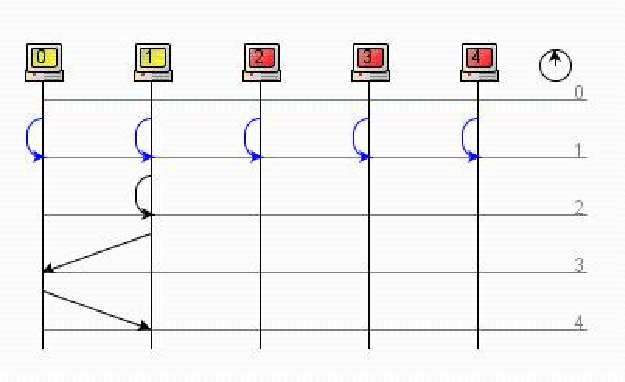
\includegraphics{images/p1ReadSeq.pdf}
	\caption{Bezeichnung der Abbildung}
	\label{a1}
\end{figure}

\begin{table} %[hbtp]
	\centering
	\begin{tabular}{l | l l l l} %Definiert Spalten der Tabelle
		\textbf{Prozesse} & \textbf{Zeit} $\rightarrow$ \\
		\hline
			$P_{1}$ & $W(x)1$ \\
			$P_{2}$ & & $W(x)2$ \\
			$P_{3}$ & & $R(x)2$ & & $R(x)1$\\
			$P_{4}$ & & & $R(x)2$ & $R(x)1$\\
	\end{tabular}
	\caption{Bezeichnung der Tabelle}
	\label{t1}
\end{table}


\section{Mathematische Formel}\index{Formel}
Mathematische Formeln bzw. Formulierungen können sowohl im laufenden Text (z.B. $y=x^2$) oder abgesetzt und zentriert im Text erscheinen. Gleichungen sollten für Referenzierungen nummeriert werden (siehe Formel \ref{gl-1}).
\begin{equation}\label{gl-1}
	e_{i}=\sum _{i=1}^{n}w_{i}x_{i}
\end{equation}

Entscheidungsformel:

\begin{equation}
	\psi(t)=\left\{
	\begin{array}{ccc}
		1 &  \qquad 0 <= t < \frac{1}{2} \\
		-1 &  \qquad \frac{1}{2} <= t <1 \\
		0 & \qquad sonst
	\end{array} \right.
\end{equation}


Matrix:\index{Matrix}
\begin{equation}
	A = \left(
	\begin{array}{llll}
		a_{11} & a_{12} & \ldots & a_{1n} \\
		a_{21} & a_{22} & \ldots & a_{2n} \\
		\vdots & \vdots & \ddots & \vdots \\
		a_{n1} & a_{n2} & \ldots & a_{nn} \\
	\end{array}
	\right)
\end{equation}

Vektor:\index{Vektor} 

\begin{equation}
	\overline{a} = \left(
	\begin{array}{c}
		a_{1}\\
		a_{2}\\
		\vdots\\
		a_{n}\\
	\end{array}
	\right)
\end{equation}

\section{Sätze, Lemmas und Definitionen}\index{Satz}\index{Lemma}\index{Definition}

Sätze, Lemmas, Definitionen, Beweise,\index{Beweis} Beispiele\index{Beispiel} können in speziell dafür vorgesehenen Umgebungen erstellt werden.

\begin{definition}(Optimierungsproblem)
	Ein \emph{Optimierungsproblem} $\mathcal{P}$ ist festgelegt durch ein Tupel
	$(I_\mathcal{P}, sol_\mathcal{P}, m_\mathcal{P}, goal)$ wobei gilt

	\begin{enumerate}
		\item $I_\mathcal{P}$ ist die Menge der Instanzen,
		\item $sol_\mathcal{P} : I_\mathcal{P} \longmapsto \mathbb{P}(S_\mathcal{P})$ ist eine Funktion, die jeder Instanz $x \in I_\mathcal{P}$ eine Menge zulässiger Lösungen zuweist,
		\item $m_\mathcal{P} : I_\mathcal{P} \times S_\mathcal{P} \longmapsto \mathbb{N}$ ist eine Funktion, die jedem Paar $(x,y(x))$ mit $x \in I_\mathcal{P}$ und $y(x) \in sol_\mathcal{P}(x)$ eine 	Zahl $m_\mathcal{P}(x,y(x)) \in \mathbb{N}$ zuordnet (= Maß für die Lösung $y(x)$ der Instanz $x$), und
		\item $goal \in \{min,max\}$.
	\end{enumerate}
\end{definition}

\begin{example} 
	MINIMUM TRAVELING SALESMAN (MIN-TSP)
	\begin{itemize}
		\item $I_{MIN-TSP} =_{def}$ s.o., ebenso $S_{MIN-TSP}$
		\item $sol_{MIN-TSP}(m,D) =_{def} S_{MIN-TSP} \cap \mathbb{N}^m$ 
		\item $m_{MIN-TSP}((m,D),(c_1, \ldots , c_m)) =_{def} \sum_{i=1}^{m-1} D(c_i, c_{i+1}) + D(c_m,c_1)$ 
		\item $goal_{MIN-TSP} =_{def} min$
	\end{itemize}
	\begin{flushright}
	$\qed$
	\end{flushright}
\end{example}

\begin{theorem} 
	Sei $\mathcal{P}$ ein \textbf{NP}-hartes Optimierungsproblem.
	Wenn $\mathcal{P} \in$ \textbf{PO}, dann ist \textbf{P} = \textbf{NP}.
\end{theorem}

\begin{proof} 
	Um zu zeigen, dass \textbf{P} = \textbf{NP} gilt, genügt es wegen Satz A.30 zu zeigen, dass ein einziges \textbf{NP}-vollständiges Problem in \textbf{P} liegt. Sei also $\mathcal{P}'$ ein beliebiges \textbf{NP}-vollständiges Problem.

	Weil $\mathcal{P}$ nach Voraussetzung \textbf{NP}-hart ist, gilt insbesondere $\mathcal{P}' \leq_T \mathcal{P}_C$. Sei $R$ der zugehörige Polynomialzeit-Algorithmus dieser Turing-Reduktion. Weiter ist $\mathcal{P} \in$ \textbf{PO} vorausgesetzt, etwa vermöge eines Polynomialzeit-Algorithmus $A$. Aus den beiden Polynomialzeit-Algorithmen $R$ und $A$ erhält man nun leicht einen effizienten Algorithmus für $\mathcal{P}'$: Ersetzt man in $R$ das Orakel durch $A$, ergibt dies insgesamt eine polynomielle Laufzeit. 
	\begin{flushright}
		$\qed$
	\end{flushright}
\end{proof}

\begin{lemma} 
	Aus \textbf{PO} $=$ \textbf{NPO} folgt \textbf{P} $=$ \textbf{NP}.
\end{lemma}

\begin{proof} 
	Es genügt zu zeigen, dass unter der angegeben Voraussetzung KNAPSACK $\in$ \textbf{P} ist.

	Nach Voraussetung ist MAXIMUM KNAPSACK $\in$ \textbf{PO}, d.h. die Berechnung von $m^*(x)$ für jede Instanz $x$ ist in Polynomialzeit möglich. Um KNAPSACK bei Eingabe $(x,k)$ zu entscheiden, müssen wir nur noch $m^*(x) \geq k$ prüfen. Ist das der Fall, geben wir $1$, sonst $0$ aus. Dies bleibt insgesamt ein Polynomialzeit-Algorithmus. 
	\begin{flushright}
		$\qed$
	\end{flushright}
\end{proof}

\section{Fußnoten}

In einer Fußnote können ergänzende Informationen\footnote{Informationen die für die Arbeit zweitrangig sind, jedoch für den Leser interessant sein könnten.} angegeben werden. Außerdem kann eine Fußnote auch Links enthalten. Wird in der Arbeit eine Software (zum Beispiel Java-API\footnote{\url{http://java.sun.com/}}) eingesetzt, so kann die Quelle, die diese Software zur Verfügung stellt in der Fußnote angegeben werden.

\section{Literaturverweise}\index{Literatur}
Alle benutzte Literatur wird im Literaturverzeichnis angegeben\footnote{Dazu wird ein sogennanter bib-File, literatur.bib verwendet.}. Alle angegebene Literatur sollte mindestens einmal im Text referenziert werden\cite{Coulouris:02}.

\chapter{Beispiel-Kapitel}
äääää
In diesem Kapitel wird beschrieben, warum es unterschiedliche Konsistenzmodelle\index{Konsistenzmodelle} gibt. Außerdem werden die Unterschiede zwischen strengen Konsistenzmodellen\index{Linearisierbarkeit} (Linearisierbarkeit, sequentielle Konsistenz)\index{sequentiell!Konsistenz} und schwachen Konsistenzmodellen\index{Konsistenz!schwach} (schwache Konsistenz, Freigabekonsistenz)\index{Freigabekonsistenz} erläutert. Es wird geklärt, was Strenge und Kosten (billig, teuer) in Zusammenhang mit Konsistenzmodellen bedeuten.

\section{Warum existieren unterschiedliche Konsistenzmodelle?}

Laut \cite{Malte:97} sind mit der\index{Replikation} Replikation von Daten immer zwei gegensätzliche Ziele verbunden: die Erhöhung der\index{Verfügbarkeit} Verfügbarkeit und die Sicherung der\index{Konsistenz} Konsistenz der Daten. Die Form der Konsistenzsicherung bestimmt dabei, inwiefern das eine Kriterium erfüllt und das andere dementsprechend nicht erfüllt ist (Trade-off zwischen Verfügbarkeit und der Konsistenz der Daten). Stark konsistente Daten sind stabil, das heißt, falls mehrere Kopien der Daten existieren, dürfen keine Abweichungen auftreten. Die Verfügbarkeit der Daten ist hier jedoch stark eingeschränkt. Je schwächer die Konsistenz wird, desto mehr Abweichungen können zwischen verschiedenen Kopien einer Datei auftreten, wobei die Konsistenz nur an bestimmten Synchronisationspunkten gewährleistet wird. Dafür steigt aber die Verfügbarkeit der Daten, weil sie sich leichter replizieren lassen.

Nach \cite{Mosberger:93} kann die Performanzsteigerung der schwächeren Konsistenzmodelle wegen der Optimierung\index{Optimierung} (Pufferung, Code-Scheduling, Pipelines) 10-40 Prozent betragen. Wenn man bedenkt, dass mit der Nutzung der vorhandenen Synchronisierungsmechanismen schwächere Konsistenzmodelle den Anforderungen der strengen Konsistenz genägen, stellt sich der höhere programmiertechnischer Aufwand bei der Implementierung der schwächeren Konsistenzmodelle als ihr einziges Manko dar.

In \cite{Cheriton:85} ist beschrieben, wie man sich Formen von DSM vorstellen könnte, für die ein beachtliches Maß an\index{Inkonsistenz} Inkonsistenz akzeptabel wäre. Beispielsweise könnte DSM verwendet werden, um die Auslastung von Computern in einem Netzwerk zu speichern, so dass Clients für die Ausführung ihrer Applikationen die am wenigsten ausgelasteten Computer auswählen können. Weil die Informationen dieser Art innerhalb kürzester Zeit ungenau werden können (und durch die Verwendung der veralteten Daten keine großen Nachteile entstehen können), wäre es vergebliche Mühe, sie ständig für alle Computer im System konsistent zu halten \cite{Coulouris:02}. Die meisten Applikationen stellen jedoch strengere Konsistenzanforderungen.

\section{Klassifizierung eines Konsistenzmodells}

Die zentrale Frage, die für die Klassifizierung\index{streng}\index{schwach} (streng oder schwach) eines Konsistenzmodells von Bedeutung ist \cite{Coulouris:02}: wenn ein Lesezugriff auf eine Speicherposition erfolgt, welche Werte von Schreibzugriffen auf diese Position sollen dann dem Lesevorgang bereitgestellt werden? Die Antwort für das schwächste Konsistenzmodell lautet: von jedem Schreibvorgang, der vor dem Lesen erfolgt ist, oder in der "`nahen"' Zukunft, innerhalb des definierten Betrachtungsraums, erfolgten wird. Also irgendein Wert, der vor oder nach dem Lesen geschrieben wurde.

Für das strengste Konsistenzmodell, Linearisierbarkeit (atomic consistency), stehen alle geschriebenen Werte allen Prozessoren sofort zur Verfügung: eine Lese-Operation gibt den aktuellsten Wert zurück, der geschrieben wurde, bevor das Lesen stattfand. Diese Definition ist aber in zweierlei Hinsicht problematisch. Erstens treten weder Schreib- noch Lese-Operationen zu genau einem Zeitpunkt auf, deshalb ist die Bedeutung von "`aktuellsten"' nicht immer klar. Zweitens ist es nicht immer möglich, genau festzustellen, ob ein Ereignis vor einem anderen stattgefunden hat, da es Begrenzungen dafür gibt, wie genau Uhren in einem verteilten System synchronisiert werden können.

Nachfolgend werden einige Konsistenzmodelle absteigend nach ihrer Strenge vorgestellt. Zuvor müssen wir allerdings klären, wie die Lese- und Schreibe-Operationen in dieser Ausarbeitung dargestellt werden.

Sei $x$ eine Speicherposition, dann können Instanzen dieser Operationen wie folgt ausgedrückt werden:
\begin{itemize}
	\item $R(x)a$ - eine Lese-Operation\index{Operation!Lese}, die den Wert $a$ von der Position $x$ liest.
	\item $W(x)b$ - eine Schreib-Operation\index{Operation!Schreib}, die den Wert $b$ an der Position $x$ speichert.
\end{itemize}

\section{Linearisierbarkeit\index{Linearisierbarkeit} (atomic consistency)}

Die Linearisierbarkeit im Zusammenhang mit DSM kann wie folgt definiert werden:
\begin{itemize}
	\item Die verzahnte Operationsabfolge findet so statt: wenn $R(x)a$ in der Folge vorkommt, dann ist die letzte Schreib-Operation, die vor ihr in der verzahnten Abfolge auftritt, $W(x)a$, oder es tritt keine Schreib-Operation vor ihr auf und $a$ ist der Anfangswert von $x$. Das bedeutet, dass eine Variable nur durch eine Schreib-Operation geändert werden kann.
	\item Die Reihenfolge der Operationen in der Verzahnung ist konsistent zu den \underline{Echtzeiten}\index{Echtzeiten}, zu denen die Operationen bei der tatsächlichen Ausführung aufgetreten sind.
\end{itemize}

Die Bedeutung dieser Definition kann an folgendem Beispiel (Tabelle \ref{tab:1}) nachvollzogen werden. Es sei angenommen, dass alle Werte mit $0$ vorinitialisiert sind.

\begin{table}
	\centering
	\begin{tabular}{l | l l l l}
		\textbf{Prozesse} & \textbf{Zeit} $\rightarrow$ & \\
		\hline
		$P_{1}$ & $W(x)1$ & & $W(y)2$ \\
		$P_{2}$ & & $R(x)1$ & & $R(y)2$ \\
	\end{tabular}
	\caption{Linearisierbarkeit ist erfüllt}
	\label{tab:1}
\end{table}

Hier sind beide Bedingungen erfüllt, da die Lese-Operationen den zuletzt geschriebenen Wert zurückliefern. Interessanter ist es, zu sehen, wann die Linearisierbarkeit verletzt ist.

\begin{table}
	\centering
	\begin{tabular}{l | l l l l}
		\textbf{Prozesse} & \textbf{Zeit} $\rightarrow$ \\
		\hline
		$P_{1}$ & $W(x)1$ & $W(x)2$ \\
		$P_{2}$ & & & \color{red} $R(x)0$ & \color{black} $R(x)2$ \\
	\end{tabular}
	\caption{Linearisierbarkeit ist verletzt, sequentielle Konsistenz ist erfüllt.}
	\label{tab:2}
\end{table}

In diesem Beispiel (Tabelle \ref{tab:2}) ist die Echtzeit-Anforderung verletzt, da der Prozess $P_{2}$ immer noch den alten Wert liest, obwohl er von Prozess $P_{1}$ bereits geändert wurde. Diese Ausführung wäre aber sequentiell konsistent (siehe kommender Abschnitt), da es eine Verzahnung der Operationen gibt, die diese Werte liefern könnte ($R(x)0$, $W(x)1$, $W(x)2$, $R(y)2$). Würde man beide Lese-Operationen des 2. Prozesses vertauschen, wie in der Tabelle \ref{tab:3} dargestellt, so wäre keine sinnvolle Verzahnung mehr möglich.

\begin{table}
	\centering
	\begin{tabular}{l | l l l l}
		\textbf{Prozesse} & \textbf{Zeit} $\rightarrow$ \\
		\hline
		$P_{1}$ & $W(x)1$ & $W(x)2$ \\
		$P_{2}$ & & & \color{red} $R(x)2$ &  \color{red} $R(x)0$ \\
			
	\end{tabular}
	\caption{Linearisierbarkeit und sequentielle Konsistenz sind verletzt.}
	\label{tab:3}
\end{table}

In diesem Beispiel sind beide Bedingungen verletzt. Selbst wenn die Echtzeit, zu der die Operationen stattgefunden haben, ignoriert wird, gibt es keine Verzahnung einzelner Operationen, die der Definition entsprechen würde.

% ...

%--------------------------------------------------------------------------
\backmatter                     %Anhang
%-------------------------------------------------------------------------
%Literaturverzeichnis - notwendig
\bibliographystyle{gerplain}
\bibliographystyle{geralpha}
\bibliography{literatur}     % BibTeX-File ist literatur.bib
%--------------------------------------------------------------------------
\printindex % Index ausdrucken - optional
%--------------------------------------------------------------------------
% Anhänge
\begin{appendix}
   \chapter{Glossar}

%geordnete tabelle, 2spaltig?
%\listofabbreviations
\abbreviation{DisASTer}		{DisASTer (Distributed Algorithms Simulation Terrain) A platform for the Implementation of Distributed Algorithms}
\abbreviation{DSM}		{		Distributed Shared Memory}
\abbreviation{AC}		{		Linearisierbarkeit (atomic consistency)}
\abbreviation{SC}		{		Sequentielle Konsistenz (sequential consistency)}
\abbreviation{WC}		{		Schwache Konsistenz (weak consistency)}
\abbreviation{RC}		{		Freigabekonsistenz (release consistency)}
 %optional  
   \chapter{Erklärung der Kandidatin / des Kandidaten}

\begin{description}[$\Box$~]
	\item[$\Box$] Die Arbeit habe ich selbständig verfasst und keine anderen als die angegebenen Quellen- und Hilfsmittel verwendet.\\

	\item[$\Box$] Die Arbeit wurde als Gruppenarbeit angefertigt. Meine eigene Leistung ist ... \\
	...\\

	Diesen Teil habe ich selbständig verfasst und keine anderen als die angegebenen Quellen und Hilfsmittel verwendet. \\

	Namen der Mitverfasser: ...

\end{description}

\vspace{2cm}

\begin{minipage}[t]{3cm}
	\rule{3cm}{0.5pt}
	Datum
\end{minipage}
\hfill
\begin{minipage}[t]{9cm}
	\rule{9cm}{0.5pt}
	Unterschrift der Kandidatin / des Kandidaten
\end{minipage}
 %optional
\end{appendix}
\end{document}
